\documentclass[11pt]{article}
\usepackage[a4paper,margin=23mm]{geometry}
\usepackage[T1]{fontenc}
\usepackage{lmodern,amsmath,amssymb,amsthm,mathtools,microtype,booktabs,graphicx}
\usepackage[colorlinks=true,linkcolor=blue,citecolor=blue,urlcolor=blue]{hyperref}
\newcommand{\EE}{\mathbb E}
\newcommand{\tr}{\operatorname{tr}}
\newcommand{\PP}{\mathcal P_H}
\newcommand{\LL}{\mathcal L}
\newcommand{\BB}{\mathcal B}
\newcommand{\Wc}{\mathcal W}
\newtheorem{theorem}{Theorem}
\title{A common-disorder algebra for two bilocal channels\\
\large Mixed-$q$ moments, actual-operator transfer and a real-time four-point function}
\author{Alan Day \and Chengheng\thanks{AI research assistant (OpenAI).}}
\date{7 November 2026\quad Local research draft}
\begin{document}\maketitle
\begin{abstract}
The charged curvature and neutral slope of the reconstructed singlet
bilocal have a joint noncommutative limit. The charged field's
two-species mixed-$q$ law was already obtained in an earlier project
stage. We identify its exact finite-size interface and add the neutral
Clifford-size residual, using source-dependent singleton normalization
and the complete local collision polynomial. The resulting three
species have effective chord lengths $(1,1,2)$. Uniform fixed moments
and strong replacement transfer this law to the actual low memory
coefficients. Their alternating four-point function and product Gram
matrix give a strictly positive, operator-valued commutator. An existing
unequal-probe kernel then supplies its real-time evolution. The full
finite-relative-time bilocal four-point function requires an additional
summable fourth-norm tail; the present result specifies that next step.
\end{abstract}

\section{Model, state and the two fields}
Use standard CAR and the overlapping complex Hermitian Gaussian
$p$-body Hamiltonian $H_N$, with the same original disorder in every
charge sector. The state is normalized annealed full-Fock trace
$\tau_N=\EE_J2^{-N}\operatorname{Tr}$ at $\beta=\mu=0$.
Take even $N$, $p\to\infty$, $\lambda_N=p^2/N\to\lambda>0$,
fixed $J_s>0$, $\hbar=1$, and string time. Put
\begin{equation}
 C=J_s^2/\lambda,\qquad q=e^{-4\lambda},\qquad
 \|X\|_r=(\tau_N|X|^r)^{1/r}.
\end{equation}
Let $Q$ be charge, $DX=QX-\sum_i c_i^\dagger Xc_i$ on neutral
operators, and $\LL\Gamma_A=|A|\Gamma_A/2$ the half-Clifford size.
With $C_Q=\EE_JH_N^2$ and $Z_2=\Wc_2(H_N^2)=H_N^2-C_Q$, define
\begin{align}
 W_{1,N}&=(p-\LL-\lambda_N)H_N,\\
 J_{2,N}&=(2p-D)Z_2-\kappa_2(H_N^2-C),
 &\kappa_2&=2\lambda\frac{1-q}{1+q}.\label{fields}
\end{align}
$W_1$ is a field, whereas $\Wc_2$ is coupling-Gaussian chaos
projection. Neither is spectral $q$-Wick ordering. Replacing
$\lambda_N$ by $\lambda$ in $W_1$ changes every fixed norm by $o(1)$.

\newpage
\section{What was already known, and its exact interface}
The previous singlet-multimark stage \cite{Old} established the
joint law of $H$ and the centered charged singlet. Its fourth moment
and its effective length two are reused here. The interface must hold
for the same disorder, not just for two matching marginal spectra.
Set
\begin{equation}
 \mathcal A=\sum_i[H,c_i]^\dagger[H,c_i],\qquad
 O=\mathcal A-\EE_J\mathcal A,\qquad
 Y^{\rm old}=O-\kappa_2Z_2.
\end{equation}
Since $DH=pH$, direct CAR expansion gives the finite-$N$ identities
\begin{align}
 \mathcal A&=(2p-D)H^2,& O&=(2p-D)Z_2,\\
 J_{2,N}-Y_N^{\rm old}&=\kappa_2(C-C_Q).\label{oldbridge}
\end{align}
$C_Q|_m=C_mI$ is a bounded deterministic charge function. Central
charge asymptotics and binomial concentration give $C_Q\to C$ in
every fixed $L^r$. Thus \eqref{oldbridge} is a strong common-sample
bridge in every fixed norm.

For the actual charge-removal compression in sector $m>0$, write
$h=H_m$, $K=I_N\otimes H_{m-1}$ and
\begin{equation}
 V\psi=m^{-1/2}\sum_i|i\rangle c_i\psi,\quad
 R=(1-VV^\dagger)KV,\quad \alpha=1-p/m.
\end{equation}
The block square gives
\begin{equation}
 mR^\dagger R=\mathcal A|_m-\frac{p^2}{m}h^2.
\end{equation}
Let $\PP$ denote samplewise energy pinching, retaining each whole
degenerate eigenspace. Charge scalars and $h^2$ commute with $h$, so
the actual zero-time dynamic memory is exactly
\begin{equation}
 \boxed{A_{0,N}=(1-\PP)mR^\dagger R=(1-\PP)J_{2,N}.}\label{A0}
\end{equation}
Inactive sectors have zero dynamic field; $m=0$ is set to zero
without using the expression containing $1/m$.

The previously proved absence of diagonal spectral mass gives
$\|\PP J_{2,N}\|_2\to0$. Old fixed high moments and pinching
contraction upgrade this to, for example,
\begin{equation}
 \|A_{0,N}-J_{2,N}\|_4
 \le\|\PP J_{2,N}\|_2^{1/3}\|J_{2,N}\|_8^{2/3}\longrightarrow0.
\end{equation}
Using any higher even norm gives the same conclusion for every
fixed finite $r$. This also recovers the old variance and fourth moment:
\begin{equation}
 w=\|J_2\|_2^2=C^2\left(4\lambda+
              \frac{16\lambda^2q}{1+q}\right),\qquad
 \tau J_2^4=(2+q^4)w^2.
\end{equation}
The new question is the joint law with $W_1$, not a new derivation
of this already recorded charged fourth moment.

\newpage
\section{Finite sources before taking the limit}
Consider a fixed trace word of pure coupling-Wick blocks, each with
one $D$ or $\LL$ mark on a disjoint region, and unmarked Hamiltonian
insertions. Internal Gaussian pairings in a pure Wick block are
forbidden. For $r$ marks use the nilpotent algebra
\begin{equation}
 \mathfrak A_r=\mathbb R[z_1,\ldots,z_r]/(z_1^2,\ldots,z_r^2).
\end{equation}
All source masks are retained. For a single-site matrix,
\begin{equation}
 D_i\begin{pmatrix}a&b\\c&d\end{pmatrix}
 =\begin{pmatrix}0&b/2\\c/2&d-a\end{pmatrix},\qquad
 \LL_i\begin{pmatrix}a&b\\c&d\end{pmatrix}
 =\frac12\begin{pmatrix}a-d&b\\c&d-a\end{pmatrix}.
\end{equation}
Multiply the complete local word in each marked region before applying
$1-z_aD_i$ or $1-z_a\LL_i$, and preserve the CAR reordering sign.
Denote its normalized trace by $T_S(z)$ for a site shared by labels $S$.
A singleton trace $t_u(z)$ has nonzero constant term $1/2$. Exact
normalization cancels the extensive marks:
\begin{equation}
 e_{\rm nil}^{\sum_a pk_az_a}\prod_u(2t_u(z))^p=1,
 \qquad R_S(z)=\epsilon_ST_S(z)\Big/\prod_{u\in S}t_u(z).
 \label{single}
\end{equation}
This division is by the source-dependent singleton, never by a
possibly zero unmarked collision trace.

\paragraph{Uniform fixed moments.}
With $2\ell$ fixed set labels, let
$R_{\rm tot}=\sum_{u<v}|I_u\cap I_v|$ and $M=\binom{2\ell}{2}$.
The coefficient norm of each local ratio is bounded by a fixed $B$.
The full normalized source word is bounded by $B^{R_{\rm tot}}$.
Hypergeometric factorial moments and H\"older give
\begin{equation}
 \EE\binom{|I_u\cap I_v|}{k}\le\frac{\lambda_N^k}{k!},
 \qquad \EE B^{R_{\rm tot}}
 \le \exp\{\lambda_+(B^M-1)\}.
\end{equation}
This proves every fixed marked moment and Schatten even-moment bound
before discarding higher intersections. Weighted triple-intersection
terms then vanish by Cauchy--Schwarz, since their probability is at
most $\binom{2\ell}{3}p^3/N^2$. Joint factorial moments identify the
remaining pair overlaps as independent Poisson variables.

For a Gaussian pairing $\pi$, the full limiting source weight is
\begin{equation}
 C^\ell e^{\lambda\kappa_\pi(z)},\qquad
 \kappa_\pi(z)=\sum_{u<v}(R_{uv}(z)-1)-\ell,
 \qquad \kappa_\pi(0)=-4\operatorname{cr}(\pi).\label{kappa}
\end{equation}
These are the BNR local-CAR/Poisson ingredients \cite{BNR}, applied
to actual common-disorder fields. The finite-$N$ domination is for
each fixed number of slots and marks; it is not a degree-uniform
bound for an infinite time series.

\newpage
\section{The neutral source and the three-species law}
A pair collision has four incidences. A marked region containing no
incidence contributes no source. A region with one incidence contains
an odd $c$ or $c^\dagger$; its factor $1-z_a/2$ cancels exactly in
\eqref{single}. Hence each surviving source needs at least two
incidences. Disjoint marked regions allow at most two such sources.
For this specified class, all source coefficients of degree three
and higher in $\kappa_\pi$ vanish. This is an extra local argument,
not a consequence of the disappearance of triple set intersections.
The complete fourth source moment is still generally nonzero:
\begin{equation}
 [z_1z_2z_3z_4]e^{\lambda(\kappa_\pi-\kappa_\pi(0))}
 =\sum_{\mathcal P\in\operatorname{Part}([4])}
       \lambda^{|\mathcal P|}\prod_{A\in\mathcal P}\kappa_A.
\end{equation}
Only singleton and pair blocks survive in this sum.

For a one-slot $W_1$ source, only collision of its own creator and
annihilator sets survives singleton cancellation. The local ratios
are $2+z_W$ with an unmarked opposite endpoint and
$2+z_W+z_{W'}+z_Wz_{W'}$ with another one-slot size mark.
With a whole-$D$ mark at the opposite endpoint the ratio remains
$2+z_W$, independent of that $D$ source. Thus
\begin{equation}
 \kappa_W=1,\quad
 \kappa_{WW'}=\mathbf1_{\text{same Gaussian chord}},\quad
 \kappa_{WD}=0.
\end{equation}
Subtracting $\lambda_NH$ removes the single-source term in the
limit. Every surviving $W$ must therefore pair directly with another
$W$, contributing $C\lambda$. Such chords are unmarked spectators
for the old $J_2$ adjacent-endpoint cancellation \cite{Old}. The
surviving charged pairs compress to length-two chords.

\begin{theorem}[Fixed words of actual low generators]
Define $h=H/\sqrt C$, $u=W_1/\sqrt{C\lambda}$ and $x=J_2/\sqrt w$.
Their limiting normalized trace moments are
\begin{equation}
 \tau(a_1\cdots a_n)=
 \sum_{\substack{\pi\in\mathcal P_2(n)\\\text{equal-species pairs}}}
       \prod_{\{e,f\}\in\operatorname{Cr}(\pi)}Q_{s(e)s(f)},
 \qquad
 Q=\begin{pmatrix}q&q&q^2\\q&q&q^2\\q^2&q^2&q^4\end{pmatrix},
 \label{law}
\end{equation}
where the species order is $(h,u,x)$. The same law holds after
replacing $J_2$ by $A_0$ and $W_1$ by $B_1/(8\lambda Cq)$.
\end{theorem}
The actual neutral replacement is proved next. The matrix in
\eqref{law} is an existing mixed-$q$ crossing matrix; a positive
tracial realization is provided by Junge--Zeng \cite{JZ}.
Our identification concerns particular same-disorder microscopic
fields. It makes no assertion of independent finite-$N$ probes.

\newpage
\section{Actual neutral slope and real-time transfer}
The neutral first coefficient from the memory expansion is
\begin{equation}
 B_{1,N}=m\epsilon_m\alpha_m(1-\PP)B_{Z,m},\quad
 B_{Z,m}=\Phi_m(h)-\bar\kappa_mh,\quad
 \epsilon_m=1-\alpha_m^2.
\end{equation}
Here $\Phi_m$ and $\bar\kappa_m$ retain their exact deterministic
sector definitions from the two-component stage \cite{Memory}.
Its full-charge $L^2$ bridge to $8\lambda CqW_1$ is already known.
To transfer four-point products one needs higher norms on both sides.

The unpinched $T_{1,m}=m\epsilon_m\alpha_mB_{Z,m}$ is a
Hermitian, $U(N)$-equivariant linear Gaussian field. Irreducibility of
$\bigwedge^m\mathbb C^N$ gives
$\EE T_{1,m}^2=v_mI$. For any such $X=\sum g_aA_a$, Gaussian
integration by parts, followed by weighted AM--GM in the eigenbasis
of $X$, gives
\begin{equation}
 \EE\tr_mX^{2k}\le(2k-1)v_m\EE\tr_mX^{2k-2}
 \le(2k-1)!!v_m^k.\label{gauss}
\end{equation}
The previous broad-central estimate
\begin{equation}
 \|B_{Z,m}\|_2\le 12C_m^{3/2}(p/N)\sqrt{K_1},\qquad
 m\epsilon_m\le2p
\end{equation}
bounds $v_m$ uniformly there. Polynomial coarse bounds in the
remaining sectors are dominated by the binomial charge tail.
Pinching is contractive and $\|1-\PP\|_{r\to r}\le2$. Thus $B_1$
has all fixed high moments. The local-source proof supplies them for
$W_1$; interpolation with the established $L^2$ bridge yields
\begin{equation}
 \boxed{\|B_{1,N}-8\lambda CqW_{1,N}\|_r\longrightarrow0
       \quad (r<\infty\text{ fixed}).}\label{B1}
\end{equation}
This argument uses linear Gaussian covariance, not a general matrix
hypercontractivity claim for higher rank descendants.

For four factors, telescoping and tracial H\"older give
\begin{equation}
 |\tau(X_1X_2X_3X_4-Y_1Y_2Y_3Y_4)|
 \le\sum_j\|X_j-Y_j\|_4
       \prod_{i\ne j}\max(\|X_i\|_4,\|Y_i\|_4).
\end{equation}
Equations \eqref{A0} and \eqref{B1} therefore transfer all fixed words
to the actual coefficients. For center-time evolution, finite unitary
insertions preserve norms. Polynomial moment convergence extends to
these insertions: bounded $C_m$ and \eqref{gauss} imply
$\|H_N\|_s\le K\sqrt s$, so the Taylor remainder satisfies
\begin{equation}
 \left\|e^{iTH_N}-\sum_{j=0}^{k}\frac{(iTH_N)^j}{j!}\right\|_r
 \le \frac{|T|^{k+1}(K\sqrt{r(k+1)})^{k+1}}{(k+1)!}\to0.
\end{equation}
Higher H\"older exponents handle the fixed field insertions. This is
uniform on compact center-time intervals and proves real-time joint
moments for the two fixed generators.

\newpage
\section{Noncommutativity and the existing real-time kernel}
Equation \eqref{law} gives
\begin{align}
 \tau(xu)&=0,&\tau(x^2u^2)&=1,&\tau(xuxu)&=q^2,\\
 \tau(u^4)&=2+q,&
 \operatorname{Gram}(xu,ux)&=
       \begin{pmatrix}1&q^2\\q^2&1\end{pmatrix}.
\end{align}
The Gram determinant is $1-q^4>0$. In particular
\begin{equation}
 \boxed{\|[x,u]\|_2^2=2(1-q^2)>0,\qquad
 \|[J_2,W_1]\|_2^2=2wC\lambda(1-q^2).}\label{comm}
\end{equation}
The commutator has zero trace and nonzero norm, so it cannot be a
scalar operator. Two-point orthogonality has not made these fields
commute. After the double-scaled limit, its normalized equal-time
squared norm is $16\lambda+O(\lambda^2)$ for small $\lambda$.

For $x(T)=e^{iTH}xe^{-iTH}$ define
\begin{equation}
 F_{xu}(T)=\tau[x(T)u\,x(T)u],\qquad
 D_{xu}(T)=\|[x(T),u]\|_2^2.
\end{equation}
The uncrossed mixed channel is $\tau[x(T)^2u^2]=1$: its two adjacent
same-species pairs cross no Hamiltonian chord, leaving cancelling
propagators. Thus $D_{xu}=2(1-F_{xu})$. Only one equal-species crossed
pairing is allowed. Use the BINT series \cite{BINT} with
$a=q^2$, $b=q$, and restore the mutual-probe weight $Q_{xu}=q^2$.
In symmetric Jacobi normalization put $\sigma=\sqrt C$ and
\begin{align}
 J_{n-1,n}&=\sigma\sqrt{\frac{1-q^n}{1-q}},&
 U(T)&=e^{-iTJ},&v_n&=U_{n0}(T),\\
 c_i&=\frac{(b^2;q)_i}{(q;q)_i}a^i,&
 V_{li}&=\sqrt{c_i}\,b^l
       \sqrt{\frac{(q;q)_{l+i}}{(q;q)_l}}v_{l+i}.
\end{align}
With $(z;q)_i=\prod_{j=0}^{i-1}(1-zq^j)$, the answer is
\begin{equation}
 \boxed{F_{xu}(T)=q^2\sum_{n,i\ge0}a^n
                 |(U(T)^\dagger V)_{ni}|^2.}\label{otoc}
\end{equation}
The formula is inherited; identifying the actual fields is the new
interface. Independent colored-chord Taylor enumeration gives
\begin{align}
 F_{xu}(T)&=q^2-2q^2(1-q)^2(1+q)(\sigma T)^2
                  +c_4(q)(\sigma T)^4+O(T^6),\\
 c_4(q)&=\frac{q^2(q-1)^3(q+1)}6
                     (9q^3+9q^2-3q-11).
\end{align}
In particular $F_{xu}(0)=q^2$. Removing the mutual factor would
incorrectly erase the equal-time commutator \eqref{comm}.

\newpage
\section{Numerical four-point function and its errors}
\begin{figure}[h!]
\centering
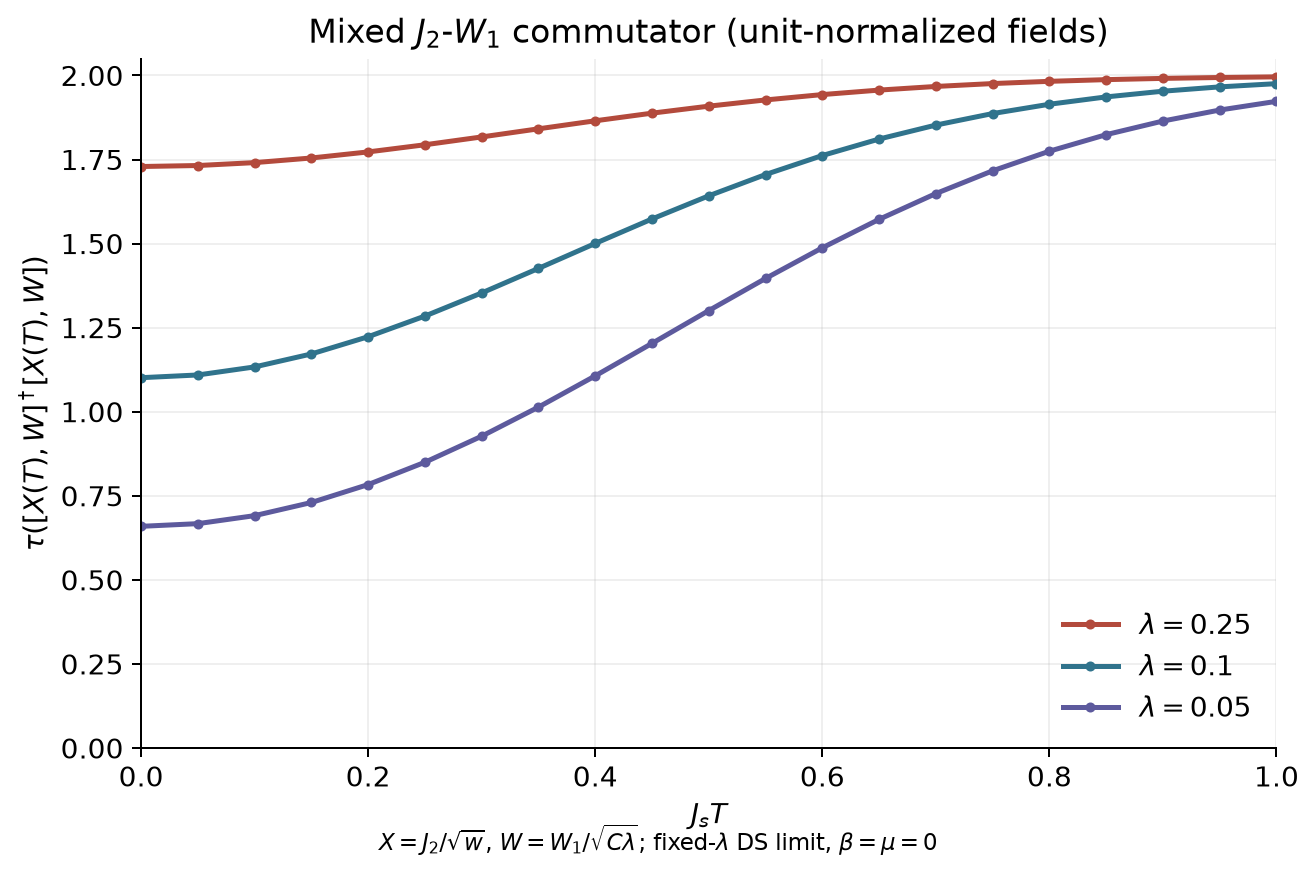
\includegraphics[width=.96\linewidth]{../../results/susskind-bilocal-four-point/normalized-commutator.png}
\caption{Real-time commutator of the two unit-normalized low channels.
The double-scaled limit is taken first at each fixed $\lambda$;
$J_s=1$. The curves do not assert a full bilocal four-point limit.}
\end{figure}
\begin{center}
\begin{tabular}{rrrr}
\toprule
$\lambda$&Jacobi cutoff $L$&$F_{xu}(1)$&$D_{xu}(1)$\\\midrule
.25&61&.00202844&1.99594313\\
.10&130&.01212498&1.97575004\\
.05&245&.03842489&1.92315023\\\bottomrule
\end{tabular}
\end{center}
There are 22 times per parameter, $0,.05,\ldots,1$ plus $.01$.
Each value is compared with cutoff $L+16$ and with exchanged probe
lengths $(1,2)$. The largest cutoff and species-swap changes are
$1.89\times10^{-15}$ and $2.23\times10^{-16}$. Independent exact
Taylor coefficients through order six use 130 arc layouts and
1,376 colored pairings per species order. The small-time numerical
comparison differs by at most $1.45\times10^{-15}$.

For analytic truncation, let $C_b=(1-q)^{-1}$, $K_b=C_b/(1-a)$,
$R_H=2\sigma/\sqrt{1-q}$ and $T_k(z)=\sum_{j\ge k}z^j/j!$.
The source map obeys $\|v\mapsto V\|\le\sqrt{K_b}$, with source
rows beyond $M$ bounded by $\sqrt{K_b}b^M$. Jacobi path agreement
below the boundary and unitarity give
\begin{equation}
 |F_{xu}-F_{xu}^{(L)}|
 \le2q^2K_b\{2T_L(R_H|T|)+2T_{L-M}(R_H|T|)+2b^M\}.
\end{equation}
The recorded interval truncation bounds are below
$5.44\times10^{-12}$. They control truncation in exact arithmetic;
the floating comparisons are not interval certificates. Saved data
include relative errors and the subtraction condition
$(1+|F|)/|1-F|$, whose maximum here is about $5.067$.

\newpage
\section{A stronger return estimate and the next target}
The previous reconstruction \cite{Reconstruction} writes the actual
dynamic bilocal as a linear filter of its actual memory, plus a
controlled return error:
\begin{equation}
 \widetilde\BB_N(t)=
 -\int_0^t ds\int_{-(t-s)/2}^{(t-s)/2}du\,
 e^{iHu}\mathcal F_N(s)e^{-iHu}\quad(t\ge0).
\end{equation}
Negative times use the adjoint relation. Its contractive background
propagator $F_0$ obeys the exact ordered identity
$F-F_0=-F_0*\delta M*F$. The old force moment theorem supplies every
fixed high norm, not just the eighth moment used in that stage.
For fixed $r\ge2$, in the good charge region $m\ge N/4$,
\begin{equation}
 \|\delta M\|_2=O(p^{-2}),\quad
 \|\delta M\|_{4r}=O(p^{-1}),\quad
 \|F-U_H\|_{2r}+\|F_0-U_H\|_{2r}=O(p^{-1}).
\end{equation}
Interpolation with $\theta=1/(2r-1)$ gives
$\|\delta M\|_{2r}=O(p^{-1-\theta})$. H\"older in the ordered
return integral, $m\le N=O(p^2)$, and the bad-charge binomial tail
therefore yield the direct extension
\begin{equation}
 \sup_{|t|\le S}\|\BB_N(t)-\widetilde\BB_N(t)\|_r
 \le K_{r,S}\{p^{-1/(2r-1)}+pe^{-N/(8r)}\}.\label{return}
\end{equation}
At $r=4$ this gives $O(p^{-1/7})$. It controls the return itself.

To pass the complete filtered field to four-point products, the next
task is a summable fourth-norm tail, for instance
\begin{equation}
 \lim_{K\to\infty}\limsup_N\sup_{|t|\le S}
 \|\widetilde\BB_N(t)-\widetilde\BB_N^{(K)}(t)\|_4=0,\label{next}
\end{equation}
with a specified finite field/degree truncation. Fixed-degree bounds
from \eqref{kappa} can grow with the degree; the old $L^2$ tail does
not yet prove \eqref{next}. Thus actual low-channel real-time
four-point convergence is established here, while the full
finite-relative-time bilocal four-point function remains open.

The physical next step is to complete that algebra and determine its
state and polarization before comparing with canonical meson dressing.
Itakura's construction \cite{Itakura} uses vacuum normal ordering,
momentum polarization and a restricted physical subspace. The current
trace and its non-scalar commutator are concrete data for that
comparison. No microscopic $P^-$, internal quark momentum fraction,
bulk mass assignment or finite-$G$ gravitational interaction is
identified by the present low-channel OTOC.

\newpage
\section{Evidence and reproducibility}
Four new scientific outputs are saved without overwriting previous
results. Analytical proofs extend the finite checks to fixed-word
limits; finite fixtures are not double-scaling fits.
\begin{itemize}
\item Complete local sources: 40,032 exact finite CAR/source coefficient
comparisons, with all sixteen masks for four marks; 4,768 collision
exponent comparisons and a separate partition expansion. There are
1,490 verified zero cubic/quartic exponent coefficients and 216
nonzero full four-mark coefficients. Negative local contributions
are retained.
\item Joint moments: 53 cyclic representatives cover 233 words,
including 23 zero representatives, four old $J_2/H$ interface checks,
and 1,763 accepted diagrams. Exact source polynomials are compared
with the compressed colored-pairing rule. Formal rational $(q,\lambda)$
checks do not impose $q=e^{-4\lambda}$ and are algebraic diagnostics.
\item Actual finite interface: three full-Fock fixtures at
$(N,p)=(2,1),(3,2),(4,2)$ give 33 exact matrix identities and 3,030
entry comparisons using rational arithmetic. The last has nonzero
commutator norm squared $73567/144$; the first two are zero controls.
Deterministic real Hermitian couplings, rather than a Gaussian
sample or a limiting normalization, test these algebraic identities.
\item Real-time kernel: 66 time points, 198 kernel evaluations,
two cutoff sizes and species exchange, with the independent Taylor
and analytic truncation checks on the preceding page.
\end{itemize}
The recorded environment is Python 3.14.5, NumPy 2.4.6, SymPy 1.14.0
and Matplotlib 3.11.0 on Windows. Parameter records, source hashes,
predecessor hashes, two compilation passes and every inspected
95-dpi final render are bound by the stage evidence file. Full
proofs are in the two companion notes on multi-source limits and
actual-operator transfer. Earlier scientific mains are not rerun.
This draft is saved locally, without a Git push or issue reply.

\begin{thebibliography}{9}\small\raggedright
\bibitem{BNR} M. Berkooz, V. Narovlansky and H. Raj,
\emph{Complex Sachdev--Ye--Kitaev model in the double scaling limit},
\href{https://arxiv.org/abs/2006.13983}{arXiv:2006.13983},
Secs.~3.2--3.3, 7 and 8.1.
\bibitem{BINT} M. Berkooz, M. Isachenkov, V. Narovlansky and G. Torrents,
\emph{Towards a full solution of the large $N$ double-scaled SYK model},
\href{https://arxiv.org/abs/1811.02584}{arXiv:1811.02584},
Sec.~4.2, Eq.~(4.10) and footnote~8.
\bibitem{JZ} M. Junge and Q. Zeng,
\emph{Ultraproduct methods for mixed $q$-Gaussian algebras},
\href{https://arxiv.org/abs/1505.07852}{arXiv:1505.07852},
Theorem~3.1 and Eq.~(3.2).
\bibitem{Old} A. Day and Chengheng, local stages
\texttt{susskind-singlet-multimark} and \texttt{susskind-mixed-cubic}
(2026): charged common-disorder moments and unequal-probe kernel.
\bibitem{Memory} A. Day and Chengheng, local stages
\texttt{susskind-memory-two-component}, \texttt{susskind-memory-size-bridge}
and \texttt{susskind-memory-joint-regression} (2026).
\bibitem{Reconstruction} A. Day and Chengheng, local stage
\texttt{susskind-bilocal-reconstruction} (2026), with the force moments
from \texttt{susskind-memory-return-expansion}.
\bibitem{Itakura} K. Itakura,
\emph{Boson Expansion Methods in (1+1)-dimensional Light-Front QCD},
\href{https://arxiv.org/abs/hep-th/9604032}{arXiv:hep-th/9604032},
Secs.~2, 4 and 5.
\end{thebibliography}
\end{document}
